%% ── Ⅰ. INTRODUCTION ─────────────────────────────────────
\chapter{Introduction}

\section{Contents of the Introduction}

The introduction consists of the research background and necessity, previous studies or theoretical background, and the objectives and contents of the study.

%% ─────────────────────────────────────────────────────────

\subsection{Function and Structure of the Introduction}

The introduction of a thesis generally has the following functions:
\begin{enumerate}[label=(\arabic*), leftmargin=3em, itemsep=0pt]
  \item To attract the reader’s interest (direct, specific, concise, and clear)
  \item To provide sufficient information for readers to understand the thesis
  \item The most important sentence is the research question
\end{enumerate}

\vspace{15mm}
\begin{figure}[htb]
    \centering
    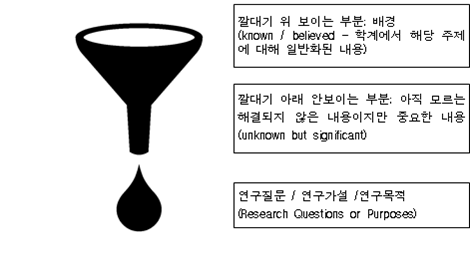
\includegraphics[width=0.7\linewidth]{images/Figure1-1.png}
    \caption{Shape of Introduction}
    \label{fig:placeholder}
\end{figure}

\subsection{Tense in the Introduction}

The tense used in the introduction generally follows these rules:
\begin{enumerate}[label=(\arabic*), leftmargin=3em, itemsep=0pt]
  \item Background or general knowledge should be written in the present tense
  \item Previous studies published by other researchers should be written in the past tense
  \item Statements indicating the research purpose or research questions are generally written in the past tense

        (The purpose of this study was to investigate \ldots)
\end{enumerate}

%% ─────────────────────────────────────────────────────────
\section{Thesis Formatting Style}

\subsection{Heading System}

Chapter numbers are written using uppercase Roman numerals. Chapter titles should use a serif font (e.g., Times New Roman) in 16pt bold and be center aligned. Subheadings should be numbered as 1.1, 1.1.1, and so on, without a period after the final number. Subheadings should use a serif font in 14pt bold and be aligned to the left.

A spacing of 10pt should be inserted below each heading line. Additional paragraph spacing can be adjusted using the paragraph settings function of the word processor.

If a heading appears at the last line of a page, extra blank space should be inserted so that the heading moves to the first line of the next page.

\subsection{Main Text}

The previous guideline specified the main text format as Times New Roman 12pt with fixed character spacing. However, for better readability, it is recommended to use 100\% character width and 0\% character spacing.

In addition, the line spacing is increased from 160\% to 200\%, and paragraph indentation is set to 10pt using the paragraph indentation function. Using manual spaces at the beginning of a paragraph is discouraged.

\subsection{Figures and Tables}

Figures and tables should be center aligned. Figure captions should be placed below the figure and centered, while table captions should be placed above the table and aligned appropriately. Captions should use a sans-serif font in 11pt bold.

Figure and table numbers should follow the ``chapter number--serial number'' format, such as Figure 2-1 and Table 2-1, without a period after the number. One blank space should be inserted between the number and the title.

Figures and tables should preferably be placed at the top or bottom of a page.

Paragraphs containing figures or tables should not be indented. Captions and contents of figures and tables are recommended to be written in English.

\vspace{10mm}
\begin{figure}[htb]
    \centering
    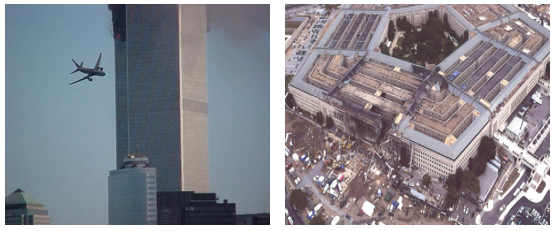
\includegraphics[width=1\linewidth]{images/Figure1-2.png}
    \caption{Title of the Figure}
    \label{fig:1-2}
\end{figure}

\begin{table}[htb]
  \caption{Title of the Table}
  \label{tab:1-1}
  \centering
  \setlength{\tabcolsep}{10pt}
  \setlength{\extrarowheight}{6pt}
  \begin{tabular}{l|l|p{2cm}|p{3cm}|p{3cm}}
    \hline
    \multicolumn{2}{l|}{} & \makecell{\textbf{Diameter}\\\textbf{(mm)}} & \makecell{\textbf{Sectional Area}\\\textbf{(mm\textsuperscript{2})}} & \makecell{\textbf{Effective Stress}\\\textbf{(MPa)}} \\
    \hline
    \multirow{2}{*}{Rebar}  & Vertical (\#14) & 43.0 & 1452 & --    \\[4pt] \cline{2-5}
                             & Hoop (\#18)     & 57.3 & 2579 & --    \\[4pt] \hline
    \multirow{2}{*}{Tendon} & Vertical        & 86.5 & 5877 & 855.8 \\[4pt] \cline{2-5}
                             & Hoop            & 86.5 & 5877 & 855.8 \\[4pt] \hline
  \end{tabular}
\end{table}

\subsection{Equations}

Equations should be center aligned, and equation numbers should be placed on the right-hand side. Equation numbers should follow the ``chapter number.serial number'' format and be enclosed in parentheses.

\begin{equation}
  \omega_1 = 2 \frac{G_F}{f_{ctm}} - 0.15 \omega_c
  \label{eq:1-1}
\end{equation}
\vspace{5mm}

A blank line may be inserted above and below equations. However, if multiple equations appear consecutively, no blank line should be inserted between them.

\subsection{Citation Style in the Main Text}

\begin{enumerate}
    \item Parenthetical citations provide brief information about referenced works within parentheses when citing another author's work in the text.

    \item Citations should include the author name and publication year within parentheses. Page numbers may also be included if necessary. If the citation appears at the end of a sentence, the period should be placed outside the parentheses. For Korean authors, both family and given names are written, whereas for foreign authors only the family name is used.

    \textbf{Examples)}
    \begin{enumerate}
        \item[a.] For a single author:
        \begin{quote}
            \ldots (Hong, 2021, pp.\ 135--146). \\
            Hong(2019) stated that \ldots \\
            Adams(2018, pp.\ 135--140) reported that \ldots
        \end{quote}

        \item[b.] For two authors:
        \begin{quote}
            Hong and Lee(2018, p.\ 35) argued that \ldots \\
            Adams and Robert(2019) suggested that \ldots
        \end{quote}

        \item[c.] For three or more authors:
        \begin{quote}
            Hong et al.(2018, pp.\ 25--28) demonstrated that \ldots \\
            Adams et al.(2020, pp.\ 25--28) reported that \ldots
        \end{quote}
    \end{enumerate}

    \item Multiple references should be separated using semicolons.

    \textbf{Example)}
    \begin{quote}
        \ldots (Hong, 2017; Lee and Lim, 2018; Adams et al., 2020).
    \end{quote}
\end{enumerate}